\lecture{11}{2025-03-24}{tri-state drivers}{}
\subsection{Tri-State Drivers}
\begin{parag}{Multiple gates driving same inputs}
    Imagine having two logic gate wanting to drive an input of a third logic gate.\\
    The issue here is the logic gates outputs should not be directly connected.
    \begin{itemize}
        \item If one gate forces '1' while the other forces '0', a low resistance path between the power supply and the ground would be created, and the resulting current would be high. We call that situation a \important{short circuit}.
    \end{itemize}
    \textbf{Solution}: Insert MUXes or tri-state drivers on the conflicting signal paths.
\end{parag}
\begin{parag}{Tris State Drivers}
    A tri-state driver has a data input, an output, and an \important{enable} input:
    \begin{center}
        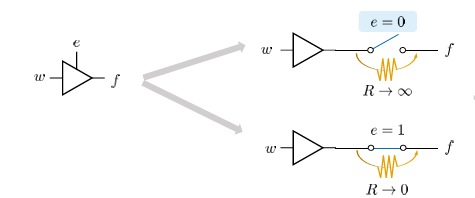
\includegraphics[scale=0.7]{12025-03-24.png}
    \end{center}
    The resulting output for this is:
    \begin{center}
    \begin{tabular}{cc|c}
        $e$ & $w$ & $f$ \\
        \hline
        \hline
        $0$ & $0$ & Z\\
        $1$ & $1$ & Z\\
        $1$ & $0$ & $0$\\
        $1$ & $1$ & $1$
    \end{tabular}
    \end{center}
    When the enable input is inactive, the output is eletrically disconnected from the data input; disconnected state is regerred to as \important{high impedance} state and usually denoted as $Z$ or $z$.
    
\begin{subparag}{Example}
    For example if we take a two gate outputs driving a wire:\\
    We need three tri-state drivers and then only one $e$ for the two tri state \important{BUT} inverted.
    \begin{center}
        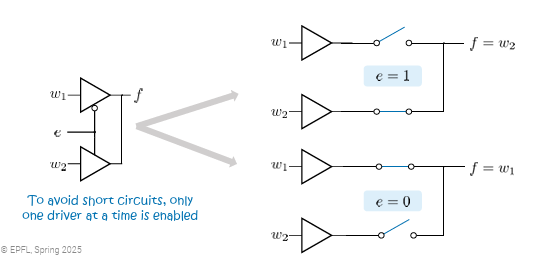
\includegraphics[scale=0.6]{22025-03-24.png}
    \end{center}
\end{subparag}
\end{parag}

\begin{parag}{Bus}
    Digital systems are commonly composed of several modules exchanging data by means of \important{common} set of interconnects (wires). \\
    The set of wires grouped under a common name is referred to as a \important{bus}
    \begin{framedremark}
        For example memory and CPU are connected with a Bus to exchange information.
    \end{framedremark}
    
    \begin{itemize}
        \item Bus receives data from several modules (one at a time) and brings that data to the inputs of other module
        \item Buses are typically $n$-bit wide, where $n > 1$
        \item Example: an $n$-bit bus DATA group $n$ wires each carrying one signal
            \begin{align*}
                DATA[0], \dots DATA[n-1
            \end{align*}
        \item In Verilog, $n$-bit and $1$-bit signals are called \important{vectors} and \important{scalars} respectively
    \end{itemize}
    This is a situation and we want to be able to implementing it.
\end{parag}
\begin{parag}{Implementing a Bus with MUXes}
    \begin{center}
        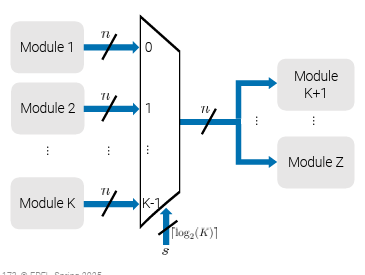
\includegraphics[scale=0.7]{42025-03-24.png}
    \end{center}
    \begin{itemize}
        \item The multiplexer takes $K$ ($k \geq 2$) n-bit data inputs and an $ \lceil \log_2 (K) \rceil$-bit select signal $s$ to select which of the inputs to pass to the output.
        \item An additional circuit that controls the activation of the \important{select} signals is typically present (which is not implemented here)
    \end{itemize}
    \begin{framedremark}
        When we have $k$ the number of select input is defined as $ \log_2(K)$,  and we rounded it up because it is defined the $2^{ \text{number of bit}}$ therefore if you take $2^{s} = K$ 
    \end{framedremark}
    
\end{parag}
\begin{parag}{Implementing a BUS with Tri-state Drivers}
    \begin{center}
        \includegraphics[scale=0.7]{52025-03-24.png}
    \end{center}
    \begin{itemize}
        \item \textbf{Only one} of the enable signals is \textbf{active} at a time so that short circuits are avoided.
        \item An additional circuit that controls the activation of the \textbf{enable} signals is typically present. (which is not implemented here)
    \end{itemize}
   
\end{parag}
\begin{parag}{Verilog Built-In Gates}
    Here is a complete list of the built in gate:
    \begin{itemize}
        \item \textbf{bufif} is a tri-state buffer
        \item \textbf{notif} is a tri-state inverter
    \end{itemize}
    \begin{center}
    \begin{tabular}{ccc}
        \hline
        and & xor & bufif0\\
        nand & xnor & bufif1\\
        or & buf & notif0\\
        nor & not & notif1
    \end{tabular}
    \end{center}
\end{parag}
\begin{parag}{Scalar  Signal Values}
    Verilog supports one-bit signal (scalars) and each individual signal can have one of the four values:
    \begin{center}
    \begin{tabular}{cc}
        \hline
        value & Meaning\\
        \hline
        $0$ & logic value $0$\\
        $1$ & logic value 1\\
        $z$ & or Z, tri-state (high impedance)\\
        $x$ & or $X$, unknown value or don't care
    \end{tabular}
    \end{center}
    Verilog support also multi-bit signal (vectors), therefore, we can specified the value of a vector by giving a constant of the form:
    \begin{align*}
        \text{[size]['radix]constant}
    \end{align*}
    Where \textit{size} is the number of bits in the constant
    \begin{center}
    \begin{tabular}{cc}
        d & decimal\\
        b & binary\\
        h & hexadecimal\\
        o & octal
    \end{tabular}
    \end{center}
   \begin{subparag}{Constants}
       If the size specifies more bits than are needed to represent the given constant, then in most casesm the constant is padded with zeors.
       \\
       the exceptions to this rule are when the first character of the constant is the either $x$ or $z$ , in which cases the padding is done using that value.
   \end{subparag}
    
\end{parag}

\begin{parag}{Concatenation Operator}
    Verilog concatenation operator $\{, \}$ allows vectos to be combined to produce a wider resulting vector:
    \begin{subparag}{Example}
        \begin{align*}
            \text{wire } [3:0] \text{ upper } = 4'b1100;\\
            \text{wire } [3:0] \text{ lower } = 4'b0011;\\
            \text{wire } [7:0] \text{ combined};
        \end{align*}
       The the result of the concatenation:
       \begin{align*}
           \text{assign } \text{ combined } = \{ \text{upper}, \text{lower}\}; \\
           = 8'b11000011
       \end{align*}
       
        
    \end{subparag}

\end{parag}
\begin{parag}{Parameters}
    parameter associate an identifier name with constant:
    \begin{subparag}{Example}
        \begin{center}
            parameter n = 4;
        \end{center}
    \end{subparag}

\end{parag}


\begin{parag}{Nets}
    Nets represent connections between circuit components, it doesn't store values, but transmit the signals. The wire are like a subclass of nets, the most common net types are $wire$ and $tri$. A wire is used to connect an output of one logic element in a circuit to an input of another logic element
    \begin{subparag}{Tri}
        The \important{tri} type denotes tri-state connections;\\
           tri nets are treated the \important{same way} as the \important{wires}; serve to enhance \important{readability} 
    \end{subparag}
\end{parag}
\subsection{Behavioral Modeling}


\begin{parag}{Example}
For instance given an input, we can label every logic gate and wrap it up into a module for instance:
\begin{center}
    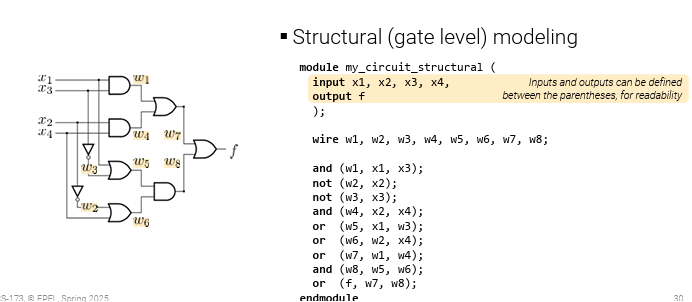
\includegraphics[scale=0.6]{12025-03-26.png}
\end{center}

\end{parag}
\begin{parag}{Behavioral modeling}

    Gate-level modeling becomes tedious for large circuit, the alternative is to use abstract expression and programming constructs to \important{ describe} the \textbf{behavior} of a logic circuit.
    \begin{center}
        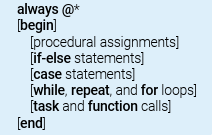
\includegraphics[scale=0.5]{22025-03-26.png}
    \end{center}
    All the operator can be use not only on the bits but on a vector.
    \begin{subparag}{Continuous assignments}
        The \important{assign} keyword provides a \important{continuous assignment for a signal}\\
        The term continuous stems from the use of Verilog in simulation of logic circuits.
        \begin{itemize}
            \item Whenever any signal on the right hand side of the assignment changes its value, the signal on the left-hand side will be re-evaluated
            \item \important{Continuous assignments are executed in parrallel}:\\
                Therefore, the order in which they appear in the code is irrelevant.
        \end{itemize}
        \begin{framedremark}
            for example, if we take $f = w7\; \mid\; w8$ whenever $w7$ or $w8$ change, $f$ \important{will be re-evaluated}.
        \end{framedremark}
    \end{subparag}
    
\end{parag}

\begin{parag}{Procedural statements}
    We can use all the \textit{"high"} level programming statements such as $if-else$, $case$, loops...\\
    hardware. However we kind of go away from the root and the "only" logic gate . Therefore, \\
    Procedural statements \important{must} be contained inside an \important{always}-block:
    \begin{itemize}
        \item Evaluated in the order given in the code.
    \end{itemize}
    To describe circuit behavior, variable are used instead of wires.
    \begin{itemize}
        \item For circuit modeling, variables of type $reg$ are used
    \end{itemize}
   
\end{parag}
\begin{parag}{Always block}
    The general format if a always block is given as:
    \begin{center}
        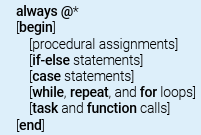
\includegraphics[scale=1]{32025-03-26.png}
    \end{center}
    \begin{framedremark}
        The square brackets indicate an optional field
    \end{framedremark}
    When multiple statements are included in the block, the begin and end keywords are needed.\\
    \textbf{always} write the (arobase)$^*$. 
\end{parag}
\begin{parag}{Full adder}
    For example if we wanted to created a full adder, we use a \textbf{case} statemants to describe the truth tables:
    \begin{center}
    \begin{tabular}{ccccc}
        x & y & $Cin$ & s & $Cout$\\
        0 & 0 & 0 & 0 & 0\\
        0 & 0 & 1 & 1 & 0\\
        0 & 1 & 0 & 1 & 0\\
        0 & 1 & 1 & 0 & 1\\
        1 & 0 & 0 & 0 & 0\\
        1 & 0 & 1 & 0 & 1\\
        1 & 1 & 0 & 0 & 1\\
        1 & 1 & 1 & 1 & 1 
    \end{tabular}
    \end{center}
Which gives us the following code:
\begin{center}
    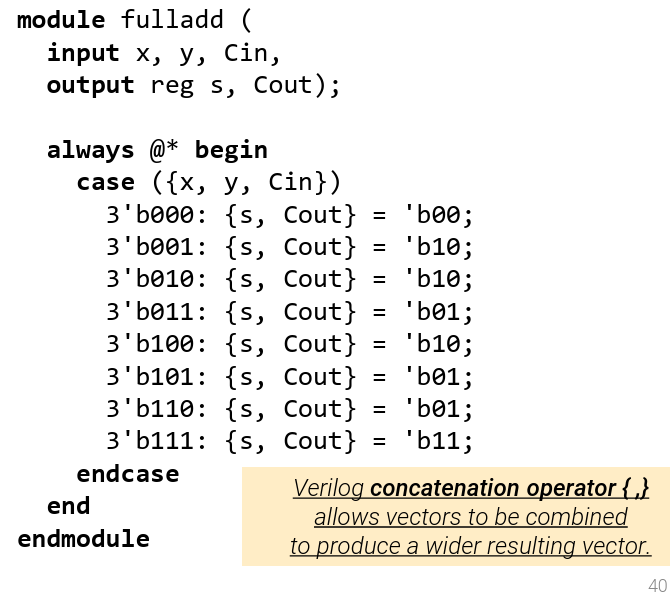
\includegraphics[scale=0.7]{42025-03-26.png}
    
\end{center}


\end{parag}




    \section{Transistors}
    There is too much schema for me to juste screenshot them and put it in the pdf, so until page 16 of the pdf Lecture -Digital Logic, Part VI, implementation technology.




